\documentclass{article}
\usepackage[english]{babel}
\usepackage{amsmath, amssymb, graphicx}
\usepackage{subfig}
\DeclareMathOperator*{\argmax}{argmax}
\graphicspath{{./images/}}


\title{CPS841 Reinforcement Learning - Assignment 3}
\author{
	Nariman Saftarli\\
	\texttt{nsaftarli@ryerson.ca}
	\and
	Nimrod Vanir\\
	\texttt{nimrod.vanir@ryerson.ca}
	}


\begin{document}
\maketitle
\newpage

\textbf{Part 1:} In Exercise 5.5, we see a 2 state MDP $s \in \{s_1, s_2\}$, $s_1$ is non-terminal, $s_2$ is terminal, and there exists a transition from $s_1$ to $s_1$ or $s_2$ with probabilities $p$ and $1-p$, respectively. The reward for every transition is $+1$. We observe a single episode lasting $10$ steps, with a return of $10$. 

For first-visit Monte-Carlo estimation for the non-terminal ($nT$) state: 
\begin{equation}
V_1(nT) = \Sigma_{i=1}^{10} \frac{i_t}{10} = \frac{10 \times 1}{10} = 1
\end{equation}

For first-visit Monte-Carlo estimation for the non-terminal ($nT$) state: 
\begin{equation}
V_n(nT) = \frac{\Sigma_{i=1}^{n} i}{n} = \frac{\Sigma_{i=1}^{10} i}{10} = \frac{55}{10} = 5.5
\end{equation}
\bigskip
\textbf{Part 2:}

The immediate difference between the Q-Learning and SARSA algorithms for this task was that the final paths produced by SARSA were closer to optimal. Since every transition rewards $-1$ other than the one to the goal state (which rewards $+100$), we can see the superiority of SARSA for this task visualized in figure 3. The average return for Q-Learning is always lower than the average return for SARSA on this task. Intuitively this makes sense since SARSA is an on-policy algorithm, and updates its value function based on the move it will take from the next state rather than the maximum value of the next state across all possible actions. Something to note is that SARSA when run with a lower value for $\alpha$ seems to get the agent on a longer streak of doing the same action over and over in states (preference for straight paths as opposed to alternating ones), suggesting that the policy is set to send the agent along the correct trajectory earlier on as opposed to using a higher $\alpha$. This makes sense as $\alpha$ is effectively a learning rate parameter, and a low value inevitably leads to better convergence, while a high one can cause sporadict movement across the error surface. 

By lowering the value of $\epsilon$ over time, we explored less and exploited more, leading to a higher average return over time. We ran our algorithms for 1000 episodes and reduced $\epsilon$ by a factor of 2 for every iteration, leading to a final value of $\frac{0.1}{2^9}$. This can be seen in Figure 6.

\begin{figure}
\begin{tabular}{ccc}
  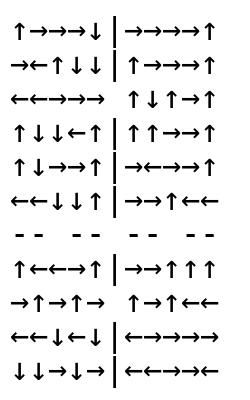
\includegraphics[scale=0.5]{q_1000_0p05_0p1.jpg} &   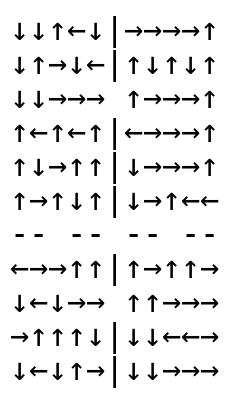
\includegraphics[scale=0.5]{q_1000_0p1_0p1.jpg} & 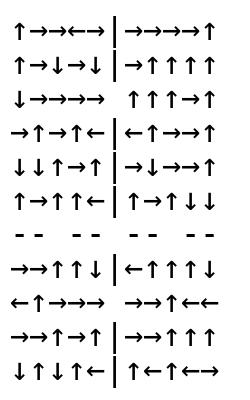
\includegraphics[scale=0.5]{q_1000_0p2_0p1.jpg} \\
  (a) $\alpha=0.05$ & (b) $\alpha=1.0$  & (c) $\alpha=2.0$\\[6pt]
  \end{tabular}
  \caption{Q-learning algorithm with values for $\alpha$ as stated above}
  \end{figure}
  
  \begin{figure}
\begin{tabular}{ccc}
  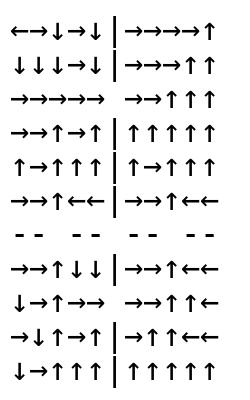
\includegraphics[scale=0.5]{sarsa_1000_0p05_0p1.jpg} &   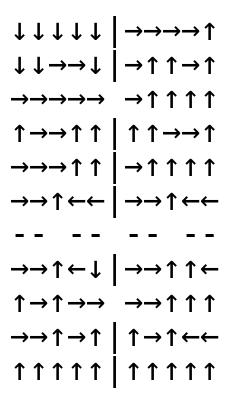
\includegraphics[scale=0.5]{sarsa_1000_0p1_0p1.jpg} & 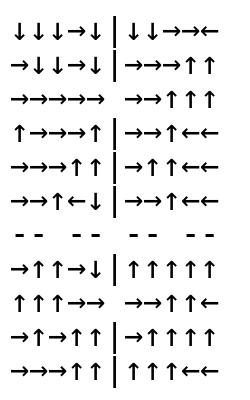
\includegraphics[scale=0.5]{sarsa_1000_0p2_0p1.jpg} \\
  (a) $\alpha=0.05$ & (b) $\alpha=1.0$  & (c) $\alpha=2.0$\\[6pt]
  \end{tabular}
  \caption{SARSA algorithm with values for $\alpha$ as stated above}
  \end{figure}

  \begin{figure}
\begin{tabular}{ccc}
  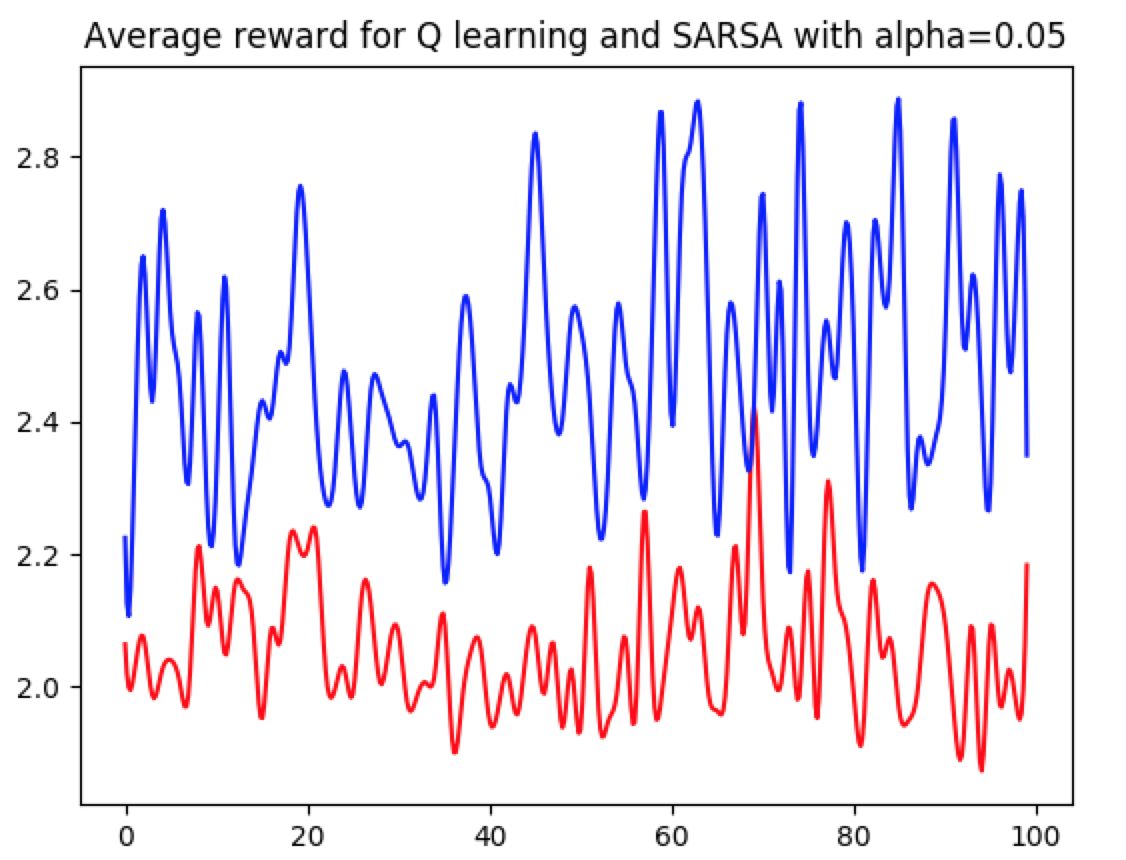
\includegraphics[scale=0.25]{avg_alpha0p05.png} &   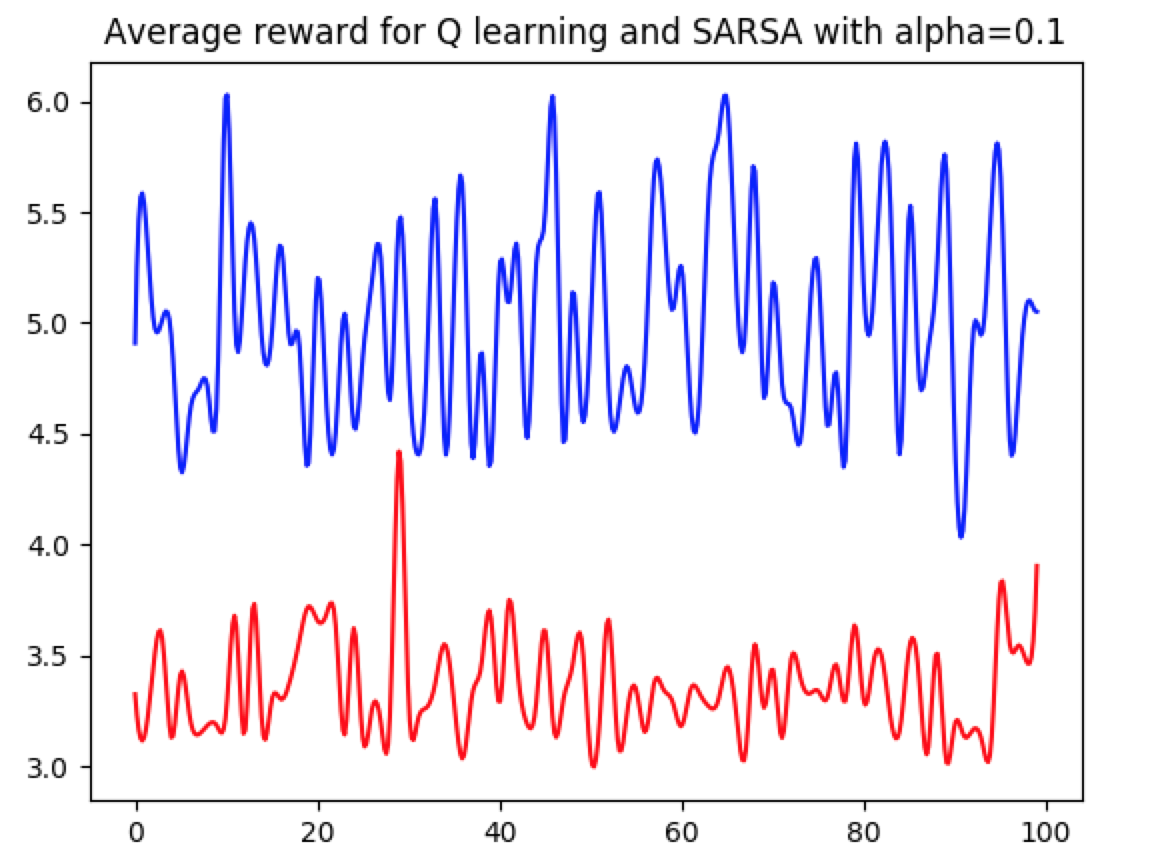
\includegraphics[scale=0.25]{avg_alpha0p1.png} & 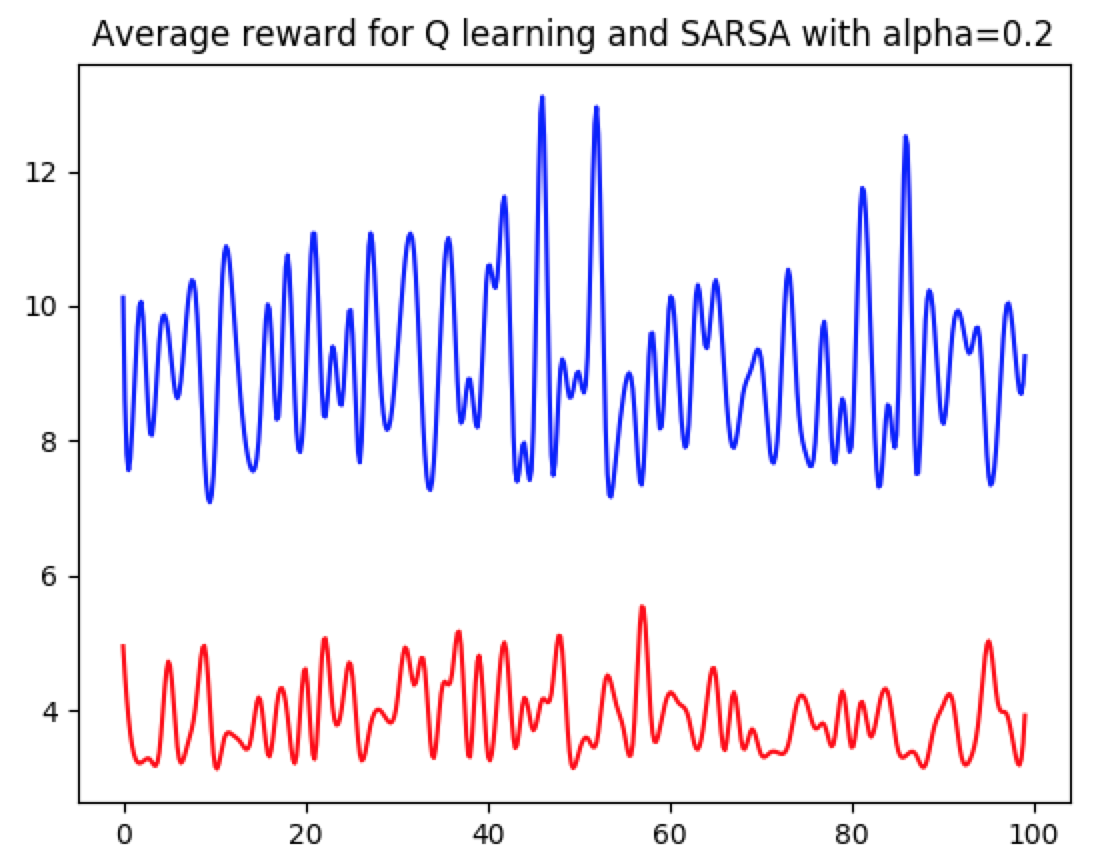
\includegraphics[scale=0.25]{avg_alpha0p2.png} \\
  (a) $\alpha=0.05$ & (b) $\alpha=1.0$  & (c) $\alpha=2.0$\\[6pt]
  \end{tabular}
  \caption{Average reward values for 100 iterations of the Q-learning algorithm (red) and SARSA (blue) with values for $\alpha$ as stated above}
  \end{figure}


  \begin{figure}
\begin{tabular}{ccc}
  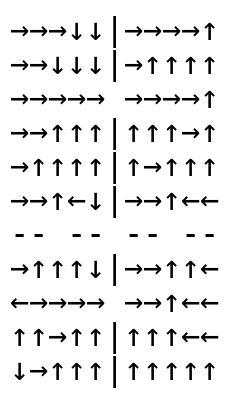
\includegraphics[scale=0.5]{sarsa_1000_0p05_0p1reduce_e.jpg} &   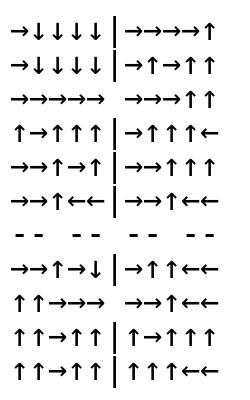
\includegraphics[scale=0.5]{sarsa_1000_0p1_0p1reduce_e.jpg} & 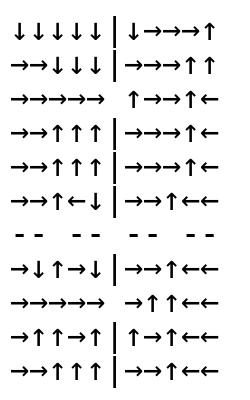
\includegraphics[scale=0.5]{sarsa_1000_0p2_0p1reduce_e.jpg} \\
  (a) $\alpha=0.05$ & (b) $\alpha=1.0$  & (c) $\alpha=2.0$\\[6pt]
  \end{tabular}
  \caption{SARSA algorithm with decreasing value of $\epsilon$ and values for $\alpha$ as stated above}
  \end{figure}

\begin{figure}
\begin{tabular}{ccc}
  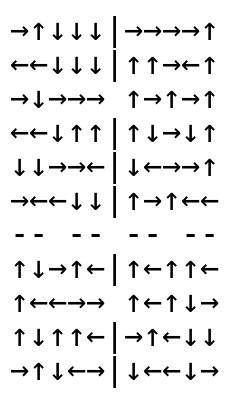
\includegraphics[scale=0.5]{q_1000_0p05_0p1reduce_e.jpg} &   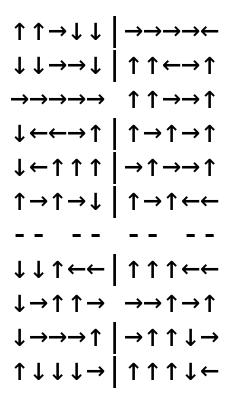
\includegraphics[scale=0.5]{q_1000_0p1_0p1reduce_e.jpg} & 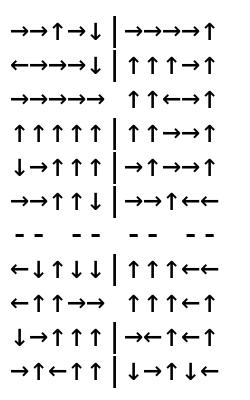
\includegraphics[scale=0.5]{q_1000_0p2_0p1reduce_e.jpg} \\
  (a) $\alpha=0.05$ & (b) $\alpha=1.0$  & (c) $\alpha=2.0$\\[6pt]
  \end{tabular}
  \caption{Q-learning algorithm with decreasing values of $\epsilon$ and values for $\alpha$ as stated above}
  \end{figure}
  
  
\begin{figure}
\begin{tabular}{ccc}
  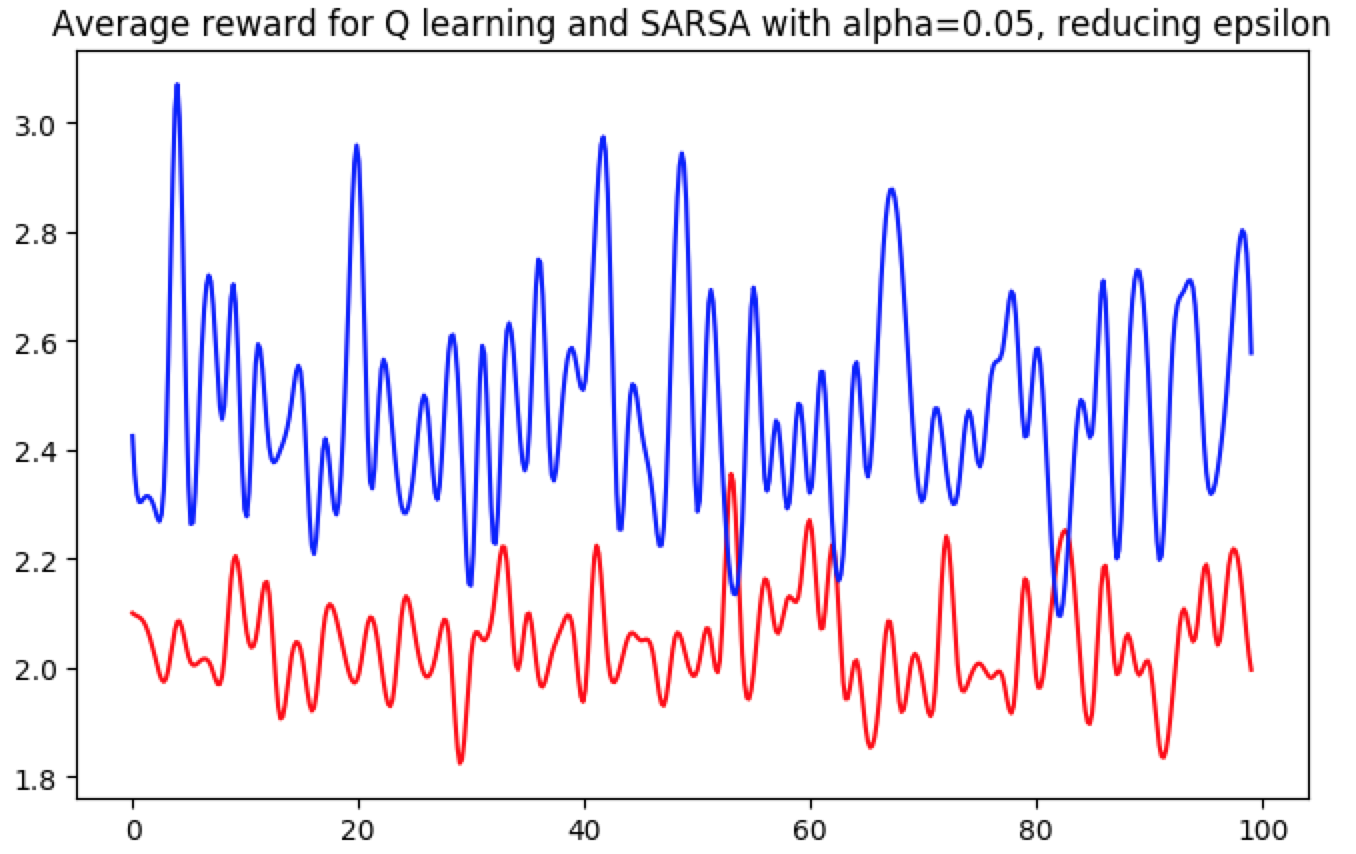
\includegraphics[scale=0.2]{avg_alpha0p05e.png} &   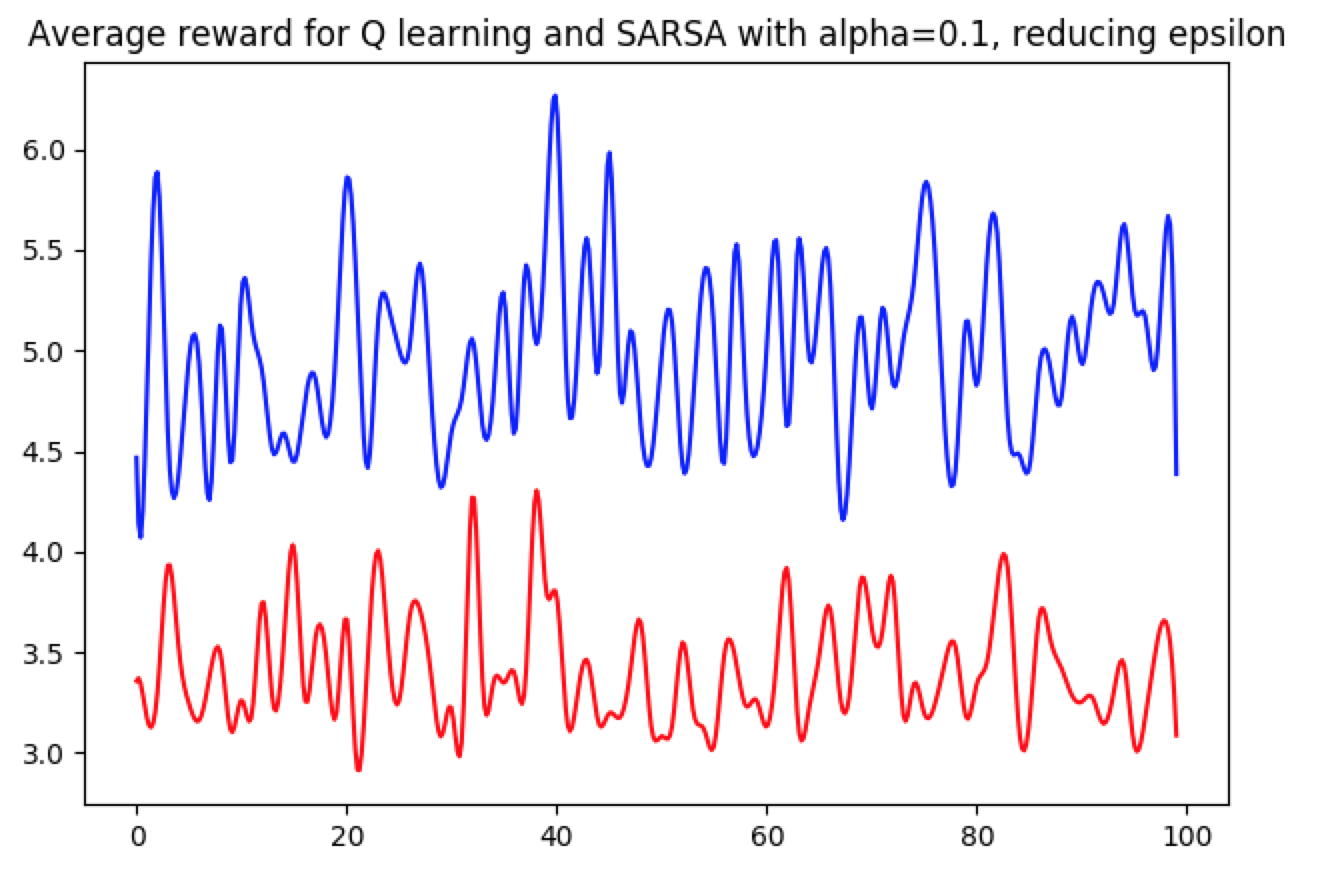
\includegraphics[scale=0.2]{avg_alpha0p1e.png} & 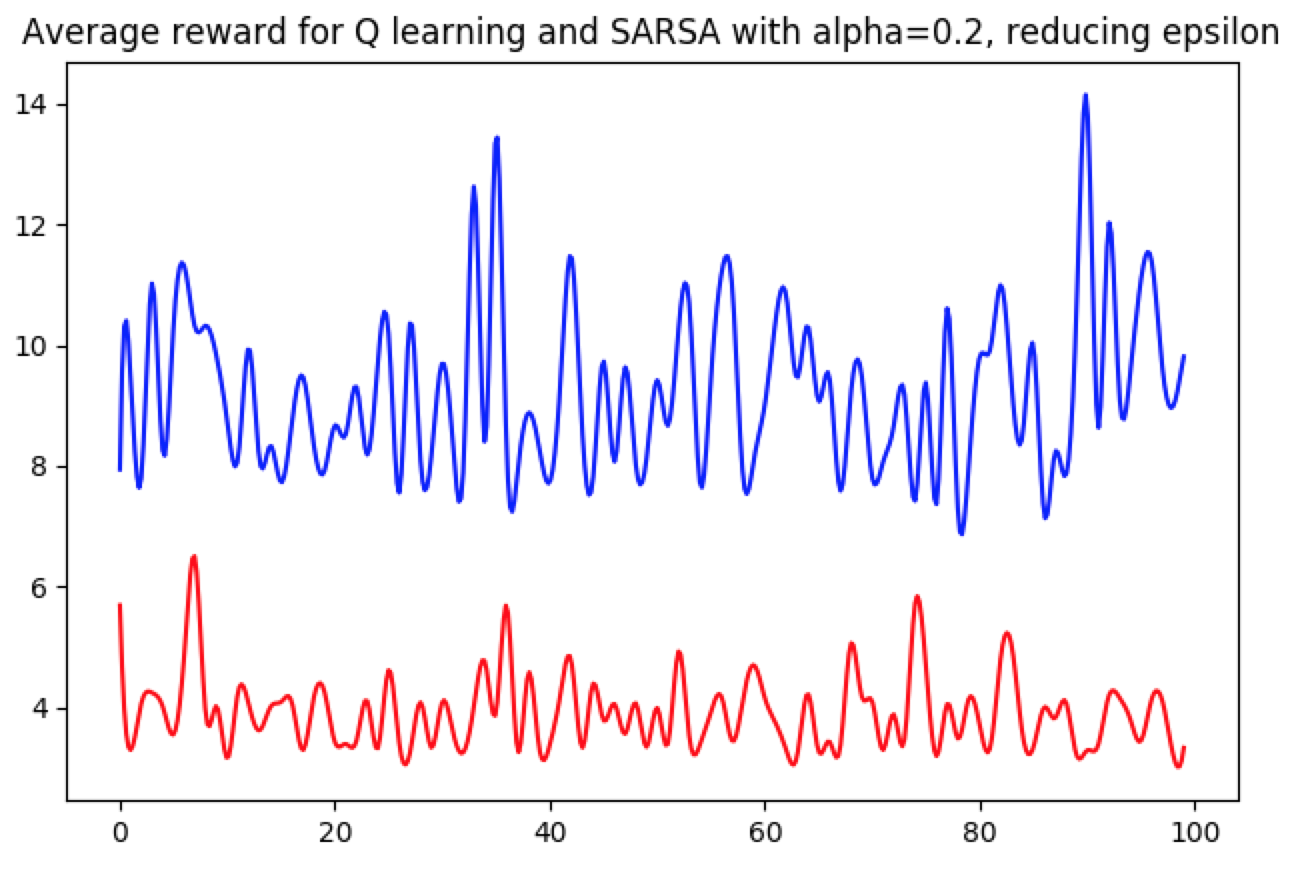
\includegraphics[scale=0.2]{avg_alpha0p2e.png} \\
  (a) $\alpha=0.05$ & (b) $\alpha=1.0$  & (c) $\alpha=2.0$\\[6pt]
  \end{tabular}
  \caption{Average reward values with decreasing $\epsilon$ for 100 iterations of the Q-learning algorithm (red) and SARSA (blue) with values for $\alpha$ as stated above}
  \end{figure}
	
	
\end{document}